
\begin{figure}[tbh]
  \centerline{
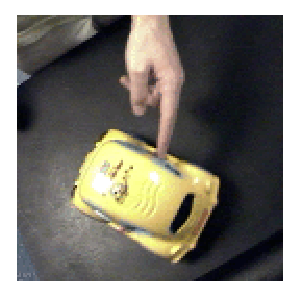
\includegraphics[width=4cm]{fig-car-hand-seg-src}
\hspace{1cm}
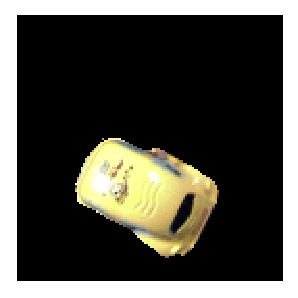
\includegraphics[width=4cm]{fig-car-hand-seg}
}
  \caption{
The segmentation algorithm will work for human poking operations, 
if the robot is fixating the object the human pokes.  The robot's 
attention system makes this a simple condition to satisfy.
}
  \label{fig:hand-poke}
\end{figure}

%%Can't necessarily remove shadow.

\section{Perceiving act{\bf ors} on objects}

\label{sect:manipulator}

Previous sections have shown how the robot can, without any prior
knowledge of their appearance, familiarize itself with objects in its
environment and its own arm.  It is possible to go still further, and
find human arms and hands in the environment, again without any prior
knowledge of their appearance.  We could imagine segmenting any moving
objects in the scene, and relying on the heuristic that hands are
often the fastest moving objects around.  A more principled approach
is to adopt an operational definition of what an arm is in terms that
the robot can perceive, just as we defined objects earlier by their
physical coherence.  Once it has poked around, the robot will be
familiar with a set of objects in its environment that are the right
scale for it to manipulate.  A reasonable definition for an arm, then,
is something that acts upon these familiar objects.  That includes the
robot's own arm, but may well include the arm of humans around the
robot. The ideal situation to detect arms is when they make contact
with a familiar object that the robot is fixating, since all the
visual processing already developed carries over without modification
(see Figure~\ref{fig:hand-poke}).  Of course the robot can easily
distinguish segmentations of its own arm from that of others simply by
whether its arm was near the target at the time!  Our experience shows
that clean segmentations of the arm (human or robot) can be extracted
as it approaches collision with a known object, when we don't need to
worry about the full complexity of human movement (see
Figure~\ref{fig:manipulator}).  But this work is still at an early stage.

%%Another approach is possible in our situation.  If the robot can
%%detect when an impact event occurs, it can collect segmentations of the
%%object that caused the impact.  The set of objects that habitually
%%trigger the motion of other objects is not a bad operational 
%%definition of a manipulator, and should include the human hand/arm,
%%and the robot's own arm.  See Figure~\ref{fig:manipulator}.

\ifverbose

Unconstrained motion in a scene is difficult to parse.  But since the
robot has become familiar with a set of objects through poking, it can
constrain the scenarios in which it may identify the manipulator.  In
particular, fixating a familiar object is a necessary condition for
reliably detecting collision.  Fixation is improved by object recognition
and localization, trained my the previous poking episodes.

May fail for more complex events -- e.g. other motion, shadows cast on
object etc.

When the robot fixates an object that it can reach, it will try to poke it.
This is inhibited if it sees motion around the object, giving a human the
opportunity to poke it instead.

The point of contact detection will still work in this case, since it 
doesn't rely on the manipulator being the robot's own arm.

The frames leading up to the impact are great for detecting the
appearance of the manipulator itself.  And give a strong cue that the
moving object is in fact a manipulator (something used to impact
objects).  See Figure~\ref{fig:manipulator}.

\fi

\begin{figure}[tbh]
  \centerline{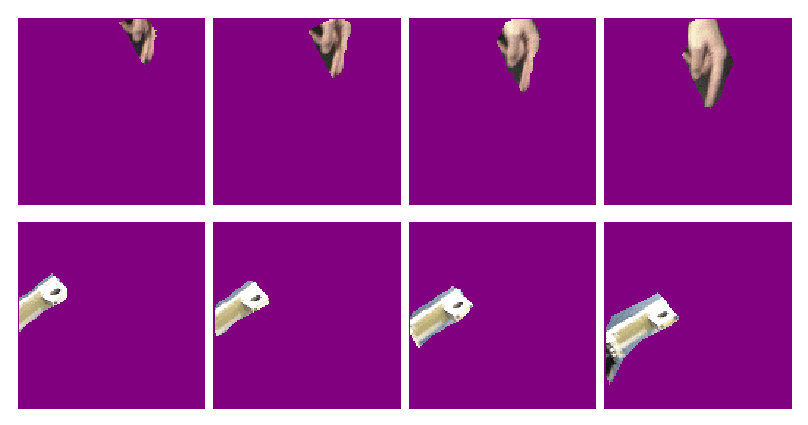
\includegraphics[width=12cm]{fig-poke-manipulator}}
%%  \centerline{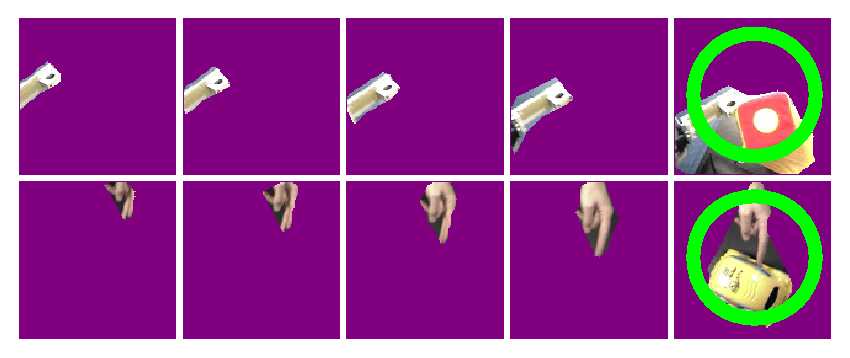
\includegraphics[width=12cm]{manipulator-segment}}
  \caption{Early experiments on segmenting the robot arm, or a 
human arm poking an object the robot.  The segmentation is
performed by working
backwards from a collision with a known object.}
  \label{fig:manipulator}
\end{figure}

